\chapter{Data Structures}

This appendix summarizes, for reference purposes, all descriptor and
block layouts in Icon.

\section{A.1 Descriptors}

Descriptors consist of two words (normally C ints): a d-word and a
v-word. The d-word contains flags in its most significant bits and
small integers in its least significant bits. The v-word contains a
value or a pointer. The flags are

\begin{tabular}{l@{\hspace{1cm}}l}
\texttt{n} & nonqualifier\\
\texttt{p} & v-word contains a pointer\\
\texttt{v} & variable\\
\texttt{t} & trapped variable\\
\end{tabular}

\subsection{A.1.1 Values}

There are three significantly different descriptor layouts for
values. A qualifier for a string is distinguished from other
descriptors by the lack of an \texttt{n} flag in its d-word, which contains
only the length of the string. For example, a qualifier for the string
{\textquotedbl}hello{\textquotedbl} is

\begin{picture}(300,40)
\put(100,0){\dvptrbox{5}{}{40}{\texttt{"hello"}}}
\end{picture}

The null value and (small) integers have type codes in their d-words and are
self-contained. Examples are:


%--%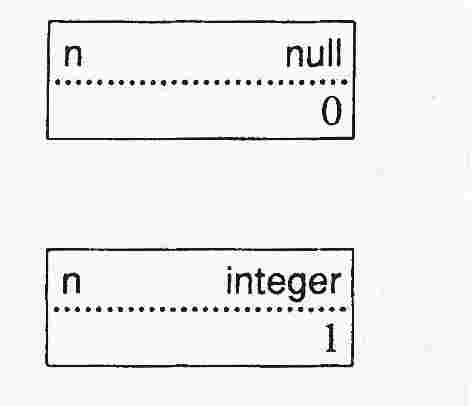
\includegraphics[width=1.602in,height=1.3547in]{ib-img/ib-img111.jpg} 
\begin{picture}(300,40)
\put(100,0){\dvbox{null}{n}{0}}
\end{picture}

\begin{picture}(300,40)
\put(100,0){\dvbox{integer}{n}{1}}
\end{picture}


For all other data types, a descriptor contains a type code in its
d-word and a pointer to a block of data in its v-word. A record is
typical:

%--%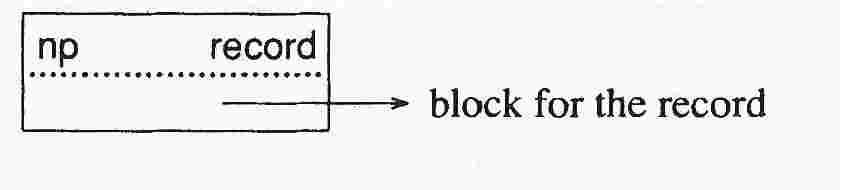
\includegraphics[width=2.8846in,height=0.6335in]{ib-img/ib-img112.jpg} 
\begin{picture}(300,40)
\put(100,0){\dvptrbox{record}{np}{40}{block for the record}}
\end{picture}

\subsection[A.1.2 Variables]{A.1.2 Variables}

There are two formats for variable descriptors. The v-word of an
ordinary variable points to the descriptor for the corresponding
value:

\begin{picture}(300,40)
\put(100,0){\dvptrbox{\textit{offset}}{npv}{40}{value descriptor}}
\end{picture}

If the variable points to a descriptor in a block, the offset is the
number of \textit{words} from the top of the block to the value
descriptor. If the variable points to a descriptor that corresponds to
an identifier, the offset is zero.


The descriptor for a trapped variable contains a type code for the
kind of trapped variable in its d-word and a pointer to the block for
the trapped variable in its v-word. The trapped variable for \texttt{\&subject}
is typical:


%--%\ \  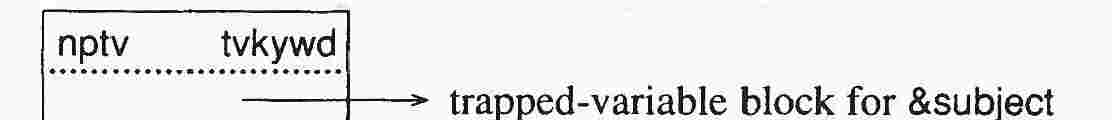
\includegraphics[width=3.7402in,height=0.4008in]{ib-img/ib-img113.jpg} 
\begin{picture}(300,40)
\put(100,0){\dvptrbox{tvkywd}{nptv}{40}{trapped-variable block for \texttt{\&subject}}}
\end{picture}

\section[A.2 Blocks]{A.2 Blocks}

With the exception of the null value, integers, and strings, the data
for Icon values is kept in blocks. The first word of every block is a
title that contains the type code for the corresponding data type. For
blocks that vary in size for a particular type, the next word is the
size of the block in bytes. The remaining words depend on the block
type, except that all non-descriptor data precedes all descriptor
data. With the exception of the long integer block, the diagrams that
follow correspond to blocks for computers with 32-bit words.

\subsection[A.2.1 Long Integers]{A.2.1 Long Integers}

%% On computers with 16-bit words, integers that are too large to fit in
%% the d-word of a descriptor are stored in blocks.  For example, the
%% block for the integer 80,000 is
An Icon integer that fits in the v-word is stored there. An integer
that is too large to fit into a word is stored in a block
that is pointed to by the v-word.
The two representations of integers are distinguished by
different internal type codes: \texttt{integer} for integers that are contained
in the v-words of their descriptors and \texttt{lrgint} for integers that are
contained in blocks pointed to by the v-words of their descriptors.
Thus, there are two internal types for one source-language data type.

%--%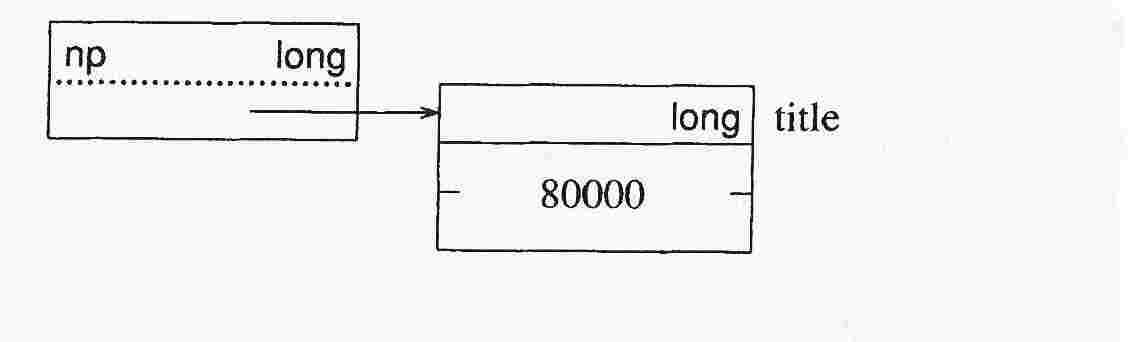
\includegraphics[width=3.848in,height=1.1425in]{ib-img/ib-img114.jpg} 
\begin{picture}(300,80)
\put(0,32){\dvptrbox{lrgint}{np}{60}{}}
\put(140,0){\blklrgbox{lrgint}{5,000,000,000}}
\put(140,17){\trboxlabel{title}}
\end{picture}

\subsection[A.2.2 Real Numbers]{A.2.2 Real Numbers}

Real numbers are represented by C doubles. For example, on computers
with 32-bit words, the real number 1.0 is represented by

%--%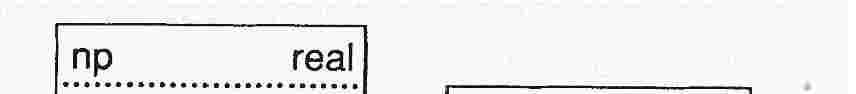
\includegraphics[width=2.8846in,height=0.3134in]{ib-img/ib-img115.jpg} 
\begin{picture}(300,80)
\put(0,32){\dvptrbox{real}{np}{60}{}}
\put(140,0){\blklrgbox{real}{1.0}}
\end{picture}

\subsection{A.2.3 Csets}

The block for a cset contains the usual type code, followed by a word
that contains the number of characters in the cset. Words totaling 256
bits follow, with a one in a bit position indicating that the
corresponding character is in the cset, and a zero indicating that it
is not. For example, \texttt{\&ascii} is

%--%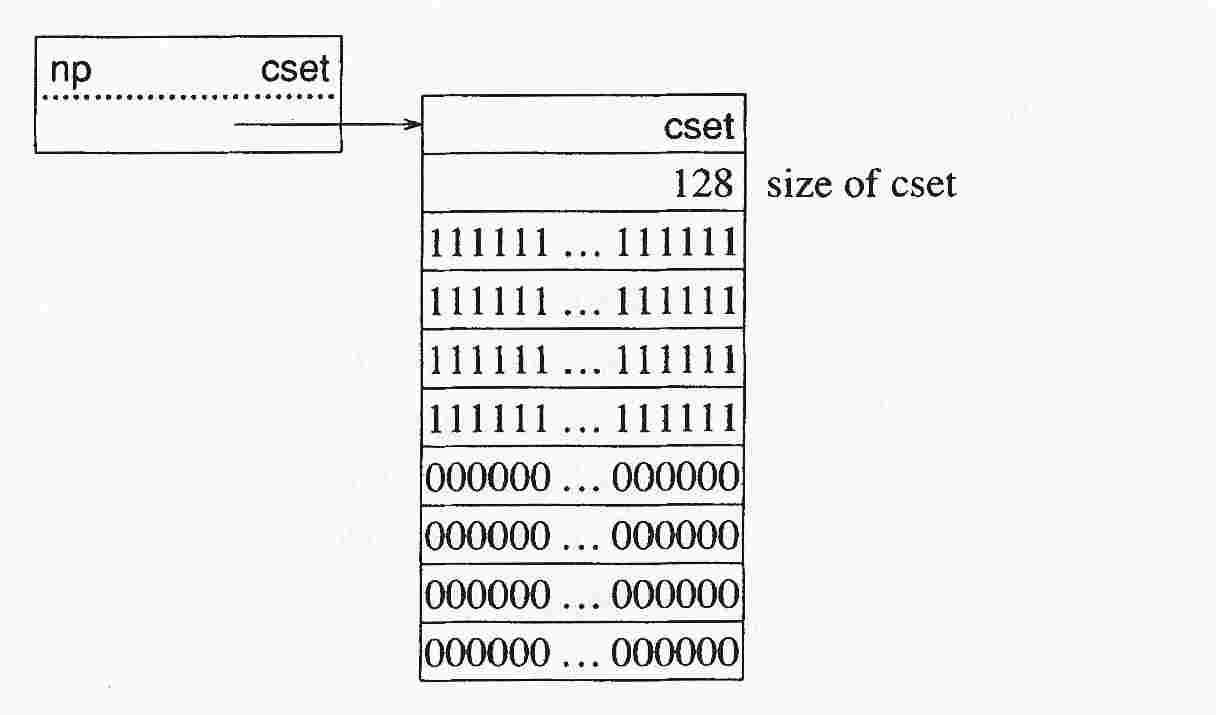
\includegraphics[width=4.0602in,height=2.3874in]{ib-img/ib-img116.jpg} 
\begin{picture}(300,200)
\put(150,0){\blkbox{000000 ... 000000}{000000 ... 000000}}
\put(150,32){\blkbox{000000 ... 000000}{000000 ... 000000}}
\put(150,64){\blkbox{111111 ... 111111}{111111 ... 111111}}
\put(150,96){\blkbox{111111 ... 111111}{111111 ... 111111}}
\put(150,128){\blkbox{cset}{128}}
\put(150,128){\brboxlabel{size of cset}}
\put(20,144){\dvptrbox{cset}{np}{50}{}}
\end{picture}

\subsection{A.2.4 Lists}

A list consists of a list-header block that points to a doubly-linked
list of list-element blocks, in which the list elements are stored in
circular queues. See Chapter 6 for details. An example is the list

%-% {\ttfamily\mdseries
%-% \ \ [1,2,3]}
\iconline{ \ \ [1,2,3] }

\noindent which is represented as

%--%\ \  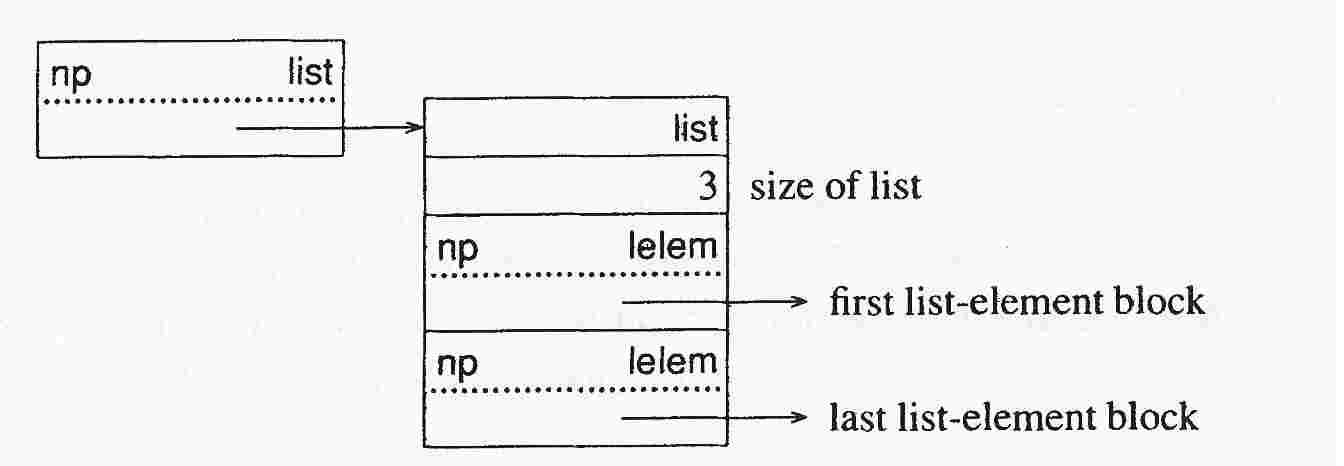
\includegraphics[width=4.489in,height=1.5563in]{ib-img/ib-img117.jpg} 
\begin{picture}(300,420)
\put(130,0){\dvbox{null}{n}{0}}
\put(130,0){\trboxlabel{slot 3}}
\put(130,32){\dvbox{integer}{n}{3}}
\put(130,32){\trboxlabel{slot 2}}
\put(130,64){\dvbox{integer}{n}{2}}
\put(130,64){\trboxlabel{slot 1}}
\put(130,96){\dvbox{integer}{n}{1}}
\put(130,96){\trboxlabel{slot 0}}
\put(130,128){\dvbox{null}{n}{0}}
\put(130,128){\trboxlabel{next list-element block}}
\put(130,160){\dvbox{null}{n}{0}}
\put(130,160){\trboxlabel{previous list-element block}}
\put(130,192){\blkbox{0}{3}}
\put(130,192){\rightboxlabels{first slot used}{number of slots used}}
\put(130,224){\blkbox{68}{4}}
\put(130,224){\rightboxlabels{size of block}{number of slots in block}}
\put(130,256){\wordbox{lelem}{}}
\put(130,288){\dvbox{lelem}{np}{}}
\put(130,288){\brboxlabel{last list-element block}}
\put(130,320){\lptr{36}}
\put(130,320){\dvbox{lelem}{np}{}}
\put(130,320){\brboxlabel{first list-element block}}
\put(130,288){\lptr{36}}
\put(114,327){\line(0,-1){64}}
\put(114,263){\vector(1,0){20}}
\put(130,352){\blkbox{list}{3}}
\put(130,352){\brboxlabel{number of elements in the list}}
\put(0,368){\dvptrbox{list}{np}{50}{}}
\end{picture}

Here there is only one list-element block:

%--%\ \  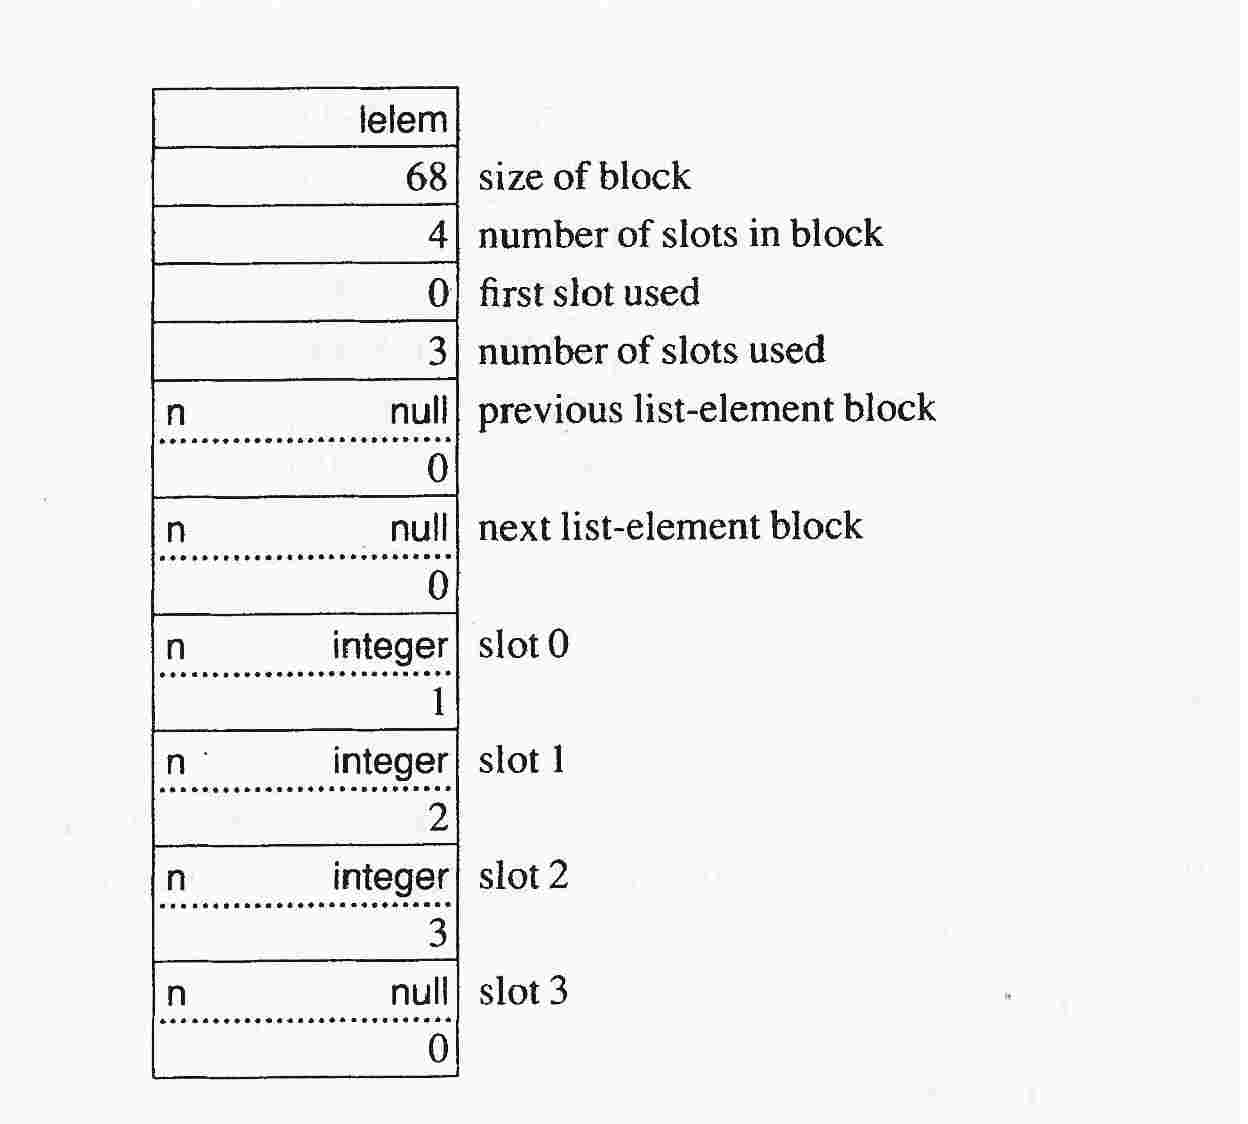
\includegraphics[width=4.1681in,height=3.7543in]{ib-img/ib-img118.jpg} 

\subsection{A.2.5 Sets}

A set consists of a set-header block that contains slots for linked
lists of set-element blocks. See Sec. 7.1 for details. An example is
given by

%-% {\ttfamily\mdseries
%-% \ \ set([1, 2, 3, 4])}
\iconline{ \ \ set([1, 2, 3, 4]) }

\noindent which is represented as

%--%\ \  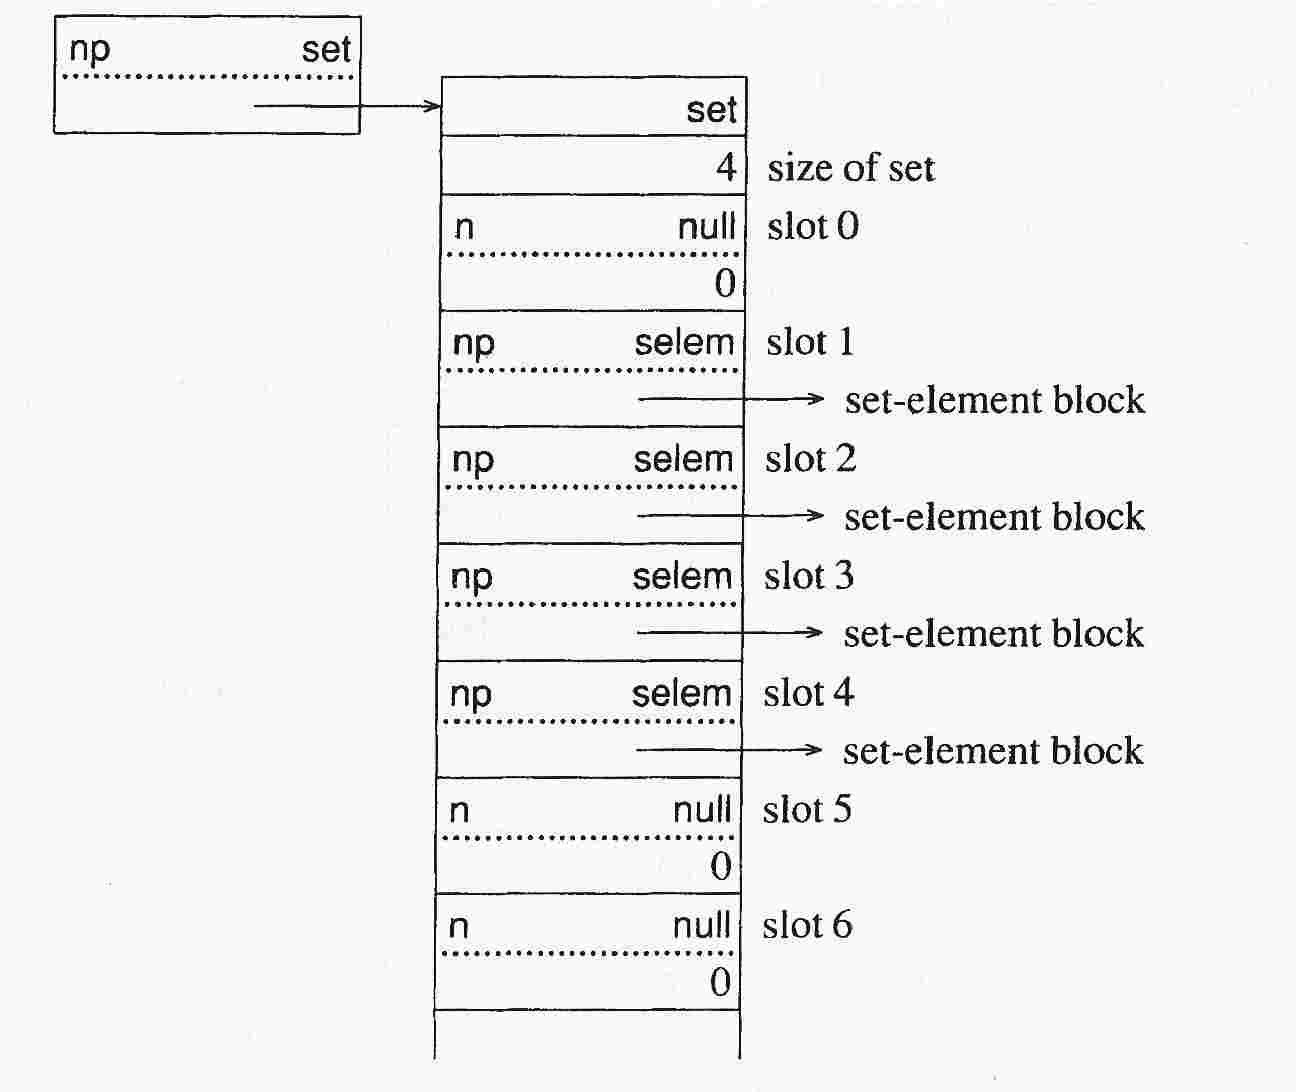
\includegraphics[width=4.3811in,height=3.6465in]{ib-img/ib-img119.jpg} 
\begin{picture}(300,300)(0,-20)
\put(130,0){\downetc}
\multiput(130,0)(0,32){2}{\dvbox{null}{n}{0}}
\multiput(130,64)(0,32){4}{\dvptrbox{selem}{np}{40}{set-element block}}
\put(130,192){\dvbox{null}{n}{0}}
\put(130,224){\blkbox{set}{4}}
\put(130,224){\brboxlabel{size of set}}
\put(130,0){\trboxlabel{slot 6}}
\put(130,32){\trboxlabel{slot 5}}
\put(130,64){\trboxlabel{slot 4}}
\put(130,96){\trboxlabel{slot 3}}
\put(130,128){\trboxlabel{slot 2}}
\put(130,160){\trboxlabel{slot 1}}
\put(130,192){\trboxlabel{slot 0}}
\put(0,240){\dvptrbox{set}{np}{50}{}}
\end{picture}

The set-element block for the member 3 is

%--%\ \  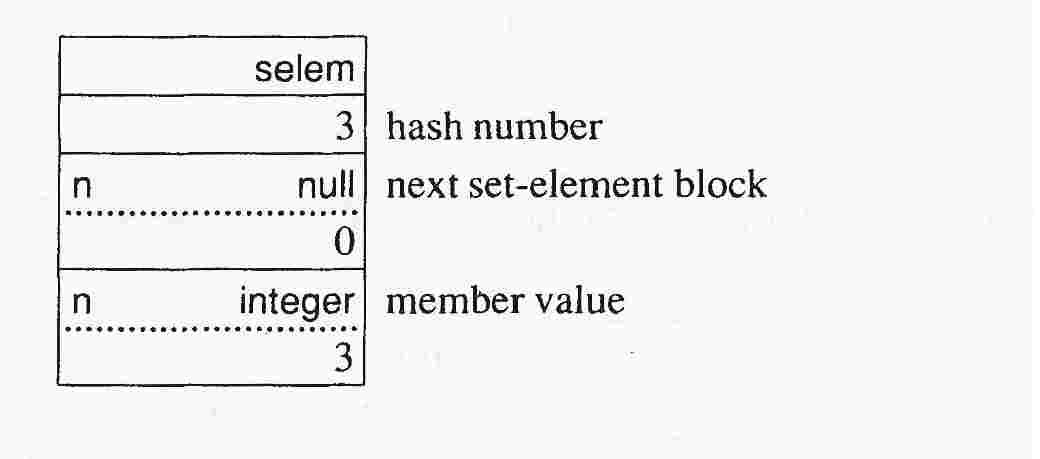
\includegraphics[width=3.5272in,height=1.5319in]{ib-img/ib-img120.jpg} 
\begin{picture}(300,100)
\put(100,0){\dvbox{integer}{n}{3}}
\put(100,0){\trboxlabel{member value}}
\put(100,32){\dvbox{null}{n}{0}}
\put(100,32){\trboxlabel{next set-element block}}
\put(100,64){\blkbox{selem}{3}}
\put(100,64){\brboxlabel{hash number}}
\end{picture}

\subsection{A.2.6 Tables}

A table is similar to a set, except that a table-header block contains
the default assigned value as well as slots for linked lists of
table-element blocks. See Sec. 7.2 for details. An example is given by

%-% {\ttfamily\mdseries
%-% \ \ t := table()}
%-% 
%-% {\ttfamily\mdseries
%-% \ \ every t[1 {\textbar} 4 {\textbar} 7] := 1}
\goodbreak
\iconcode{
\>t := table()\\
\>every t[1 | 4 | 7] := 1
}

The table \texttt{t} is represented as

%--%\ \  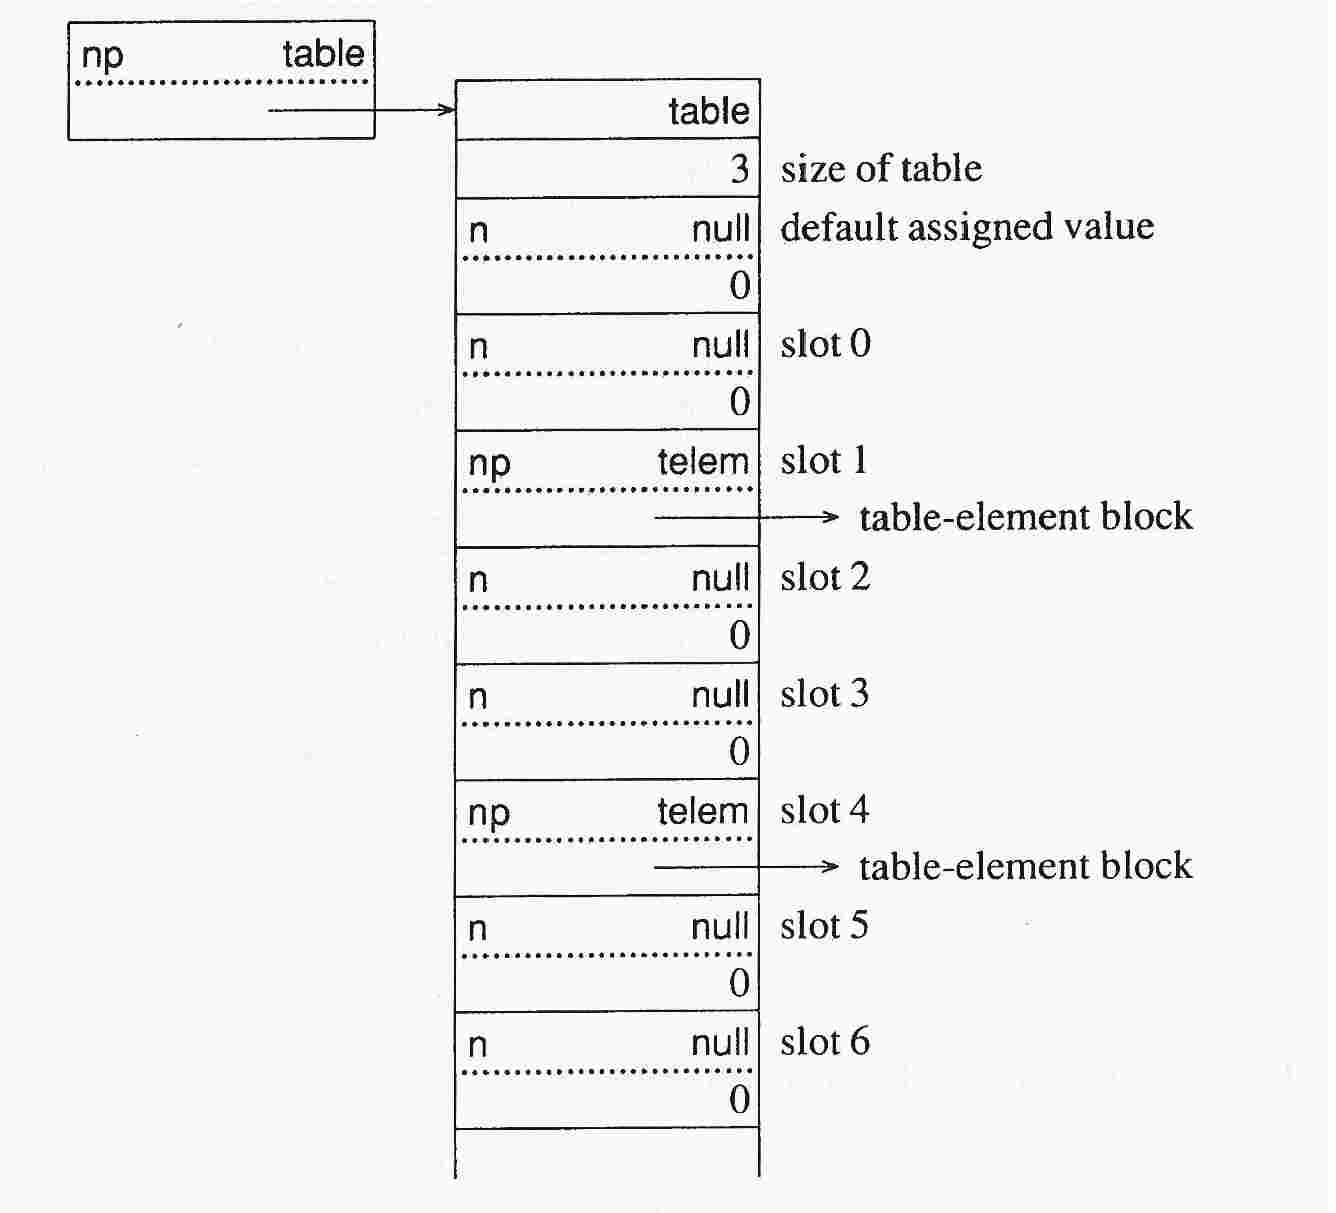
\includegraphics[width=4.489in,height=4.0516in]{ib-img/ib-img121.jpg} 
\begin{picture}(300,330)(0,-32)
\put(130,0){\downetc}
\multiput(130,0)(0,96){2}{
\begin{picture}(0,0)(4,0)
\put(0,0){\dvbox{null}{n}{0}}
\put(0,32){\dvbox{null}{n}{0}}
\put(0,64){\dvptrbox{telem}{np}{40}{table-element block}}
\end{picture}
}
\put(130,192){\dvbox{null}{n}{0}}
\put(130,224){\dvbox{null}{n}{0}}
\put(130,224){\brboxlabel{default assigned value}}
\put(130,256){\blkbox{table}{3}}
\put(130,256){\brboxlabel{size of table}}
\put(0,272){\dvptrbox{table}{np}{50}{}}
\put(130,0){\trboxlabel{slot 6}}
\put(130,32){\trboxlabel{slot 5}}
\put(130,64){\trboxlabel{slot 4}}
\put(130,96){\trboxlabel{slot 3}}
\put(130,128){\trboxlabel{slot 2}}
\put(130,160){\trboxlabel{slot 1}}
\put(130,192){\trboxlabel{slot 0}}
\end{picture}

The table-element block for the entry value 4 in the previous example is


%--%\ \  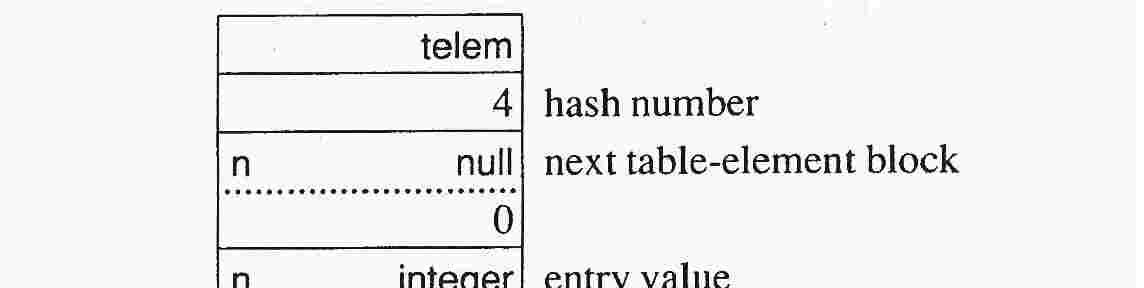
\includegraphics[width=3.848in,height=0.961in]{ib-img/ib-img122.jpg} 
\begin{picture}(300,140)
\put(100,0){\dvbox{integer}{n}{1}}
\put(100,0){\trboxlabel{assigned value}}
\put(100,32){\dvbox{null}{n}{0}}
\put(100,32){\trboxlabel{entry value}}
\put(100,64){\dvbox{null}{n}{0}}
\put(100,64){\trboxlabel{next table-element block}}
\put(100,96){\blkbox{telem}{4}}
\put(100,96){\brboxlabel{hash number}}
\end{picture}

\subsection[A.2.7 Procedures]{A.2.7 Procedures}

The procedure blocks for procedures and functions are similar. For a
procedure declaration such as

%-% {\ttfamily\mdseries
%-% \ \ procedure calc(i,gj)}
%-% 
%-% {\ttfamily\mdseries
%-% \ \ local k}
%-% 
%-% {\ttfamily\mdseries
%-% \ \ static base, index}
%-% 
%-% {\ttfamily\mdseries
%-% \ \ end}
\goodbreak
\iconcode{
procedure calc(i,gj)\\
\>local k\\
\>static base, index\\
\>\>\vdots\\
end
}

\noindent the procedure block is


%--%\ \  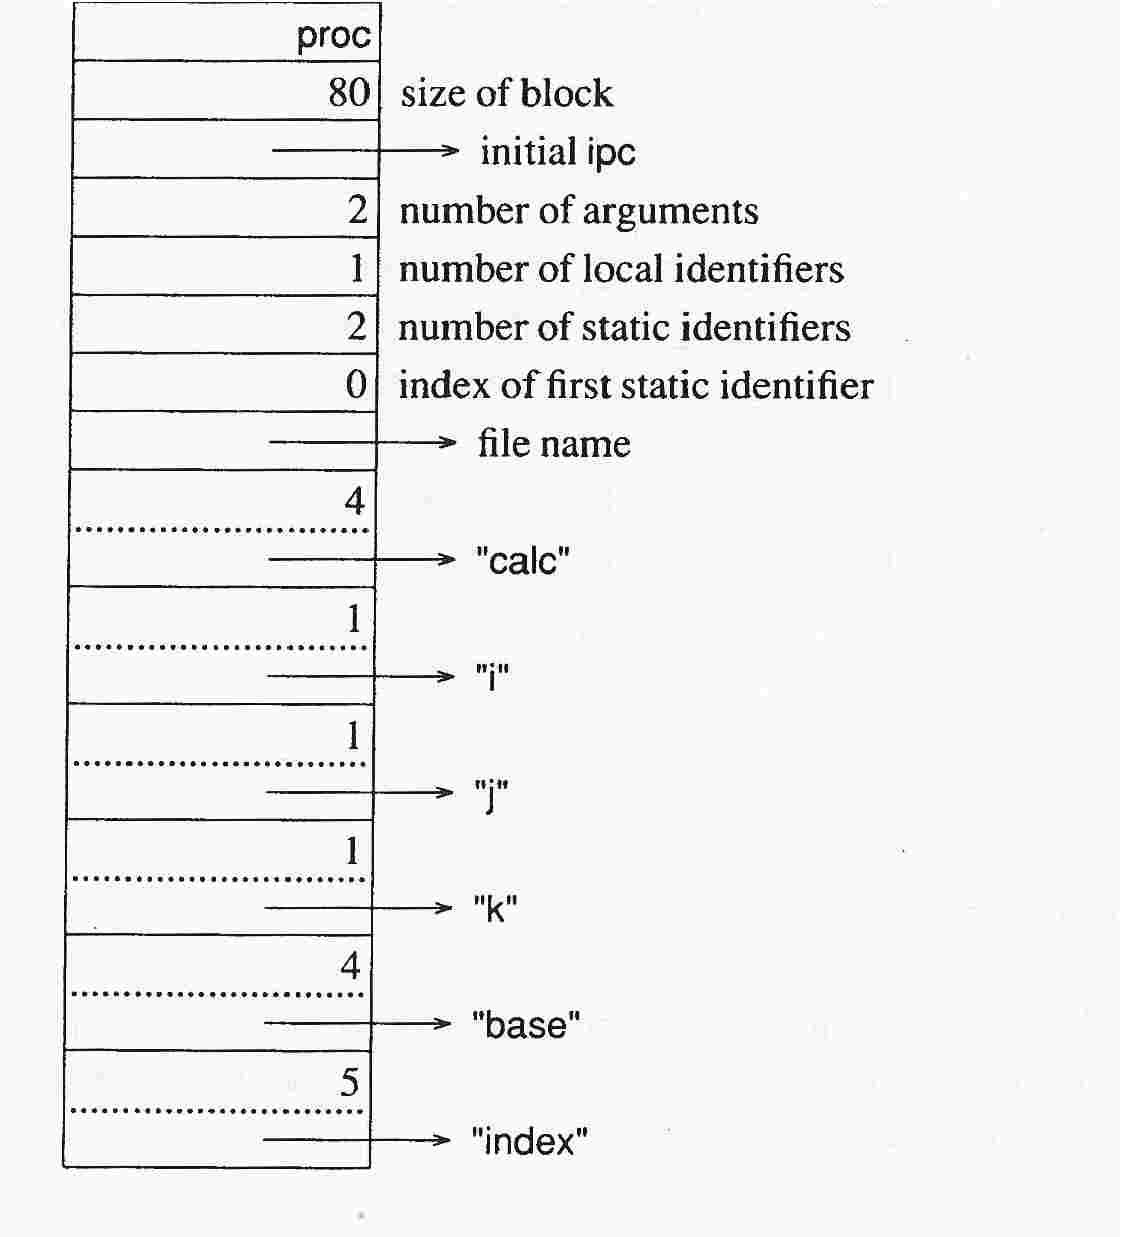
\includegraphics[width=3.848in,height=4.1307in]{ib-img/ib-img123.jpg} 
\begin{picture}(300,340)
\begin{picture}(0,0)(-100,-192)
\put(0,0){\blkptrbox{0}{40}{file name}}
\put(0,0){\trboxlabel{index of first static identifier}}
\put(0,32){\blkbox{1}{2}}
\put(0,32){\rightboxlabels{number of local identifiers}{number of static identifiers}}
\put(0,64){\wordbox{2}{}}
\put(0,64){\brboxlabel{number of arguments}}
\put(0,80){\blkptrbox{80}{40}{initial ipc}}
\put(0,80){\trboxlabel{size of block}}
\put(0,112){\wordbox{proc}{}}
\end{picture}
\put(100,0){\dvptrbox{5}{}{40}{"index"}}
\put(100,32){\dvptrbox{4}{}{40}{"base"}}
\put(100,64){\dvptrbox{1}{}{40}{"k"}}
\put(100,96){\dvptrbox{1}{}{40}{"j"}}
\put(100,128){\dvptrbox{1}{}{40}{"i"}}
\put(100,160){\dvptrbox{4}{}{40}{"calc"}}
\end{picture}


In a procedure block for a function, there is a value of -1 in place
of the number of dynamic locals. For example, the procedure block for
\texttt{repl} is


%--%\ \  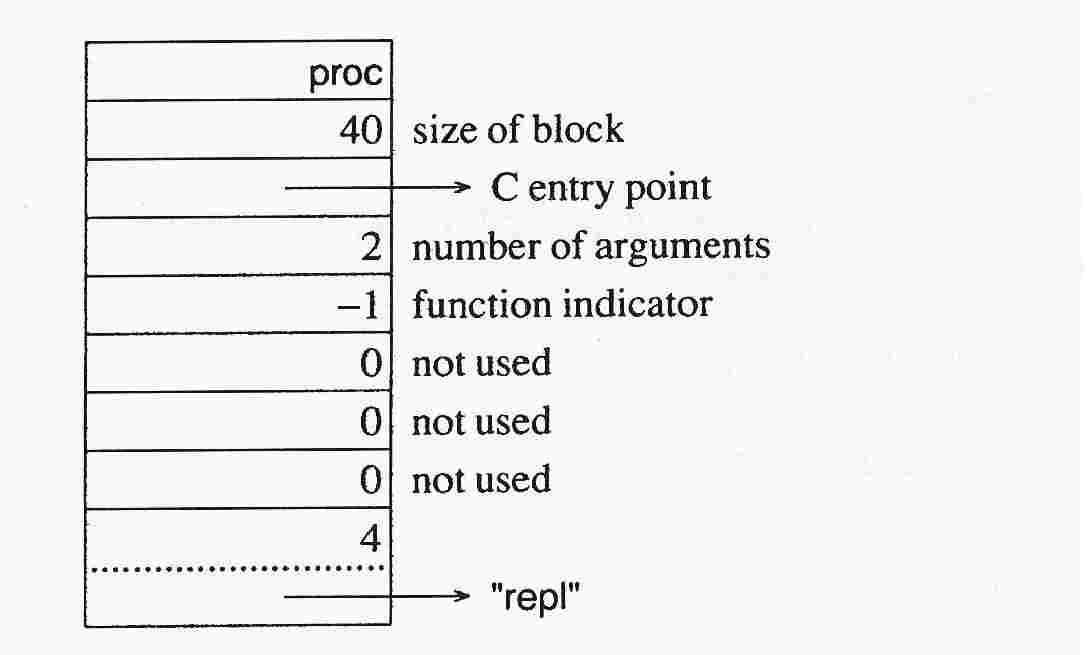
\includegraphics[width=3.6335in,height=2.1866in]{ib-img/ib-img124.jpg} 
\begin{picture}(300,170)
\begin{picture}(0,0)(-100,-32)
\put(0,0){\blkbox{0}{0}}
\put(0,0){\rightboxlabels{not used}{not used}}
\put(0,32){\blkbox{-1}{0}}
\put(0,32){\rightboxlabels{function indicator}{not used}}
\put(0,64){\wordbox{2}{}}
\put(0,64){\brboxlabel{number of arguments}}
\put(0,80){\blkptrbox{40}{40}{C entry point}}
\put(0,80){\trboxlabel{size of block}}
\put(0,112){\wordbox{proc}{}}
\end{picture}
\put(100,0){\dvptrbox{4}{}{40}{"repl"}}
\end{picture}


In the case of a function, such as \texttt{write}, which has a variable number
of arguments, the number of arguments is given as -1:


%--%\ \  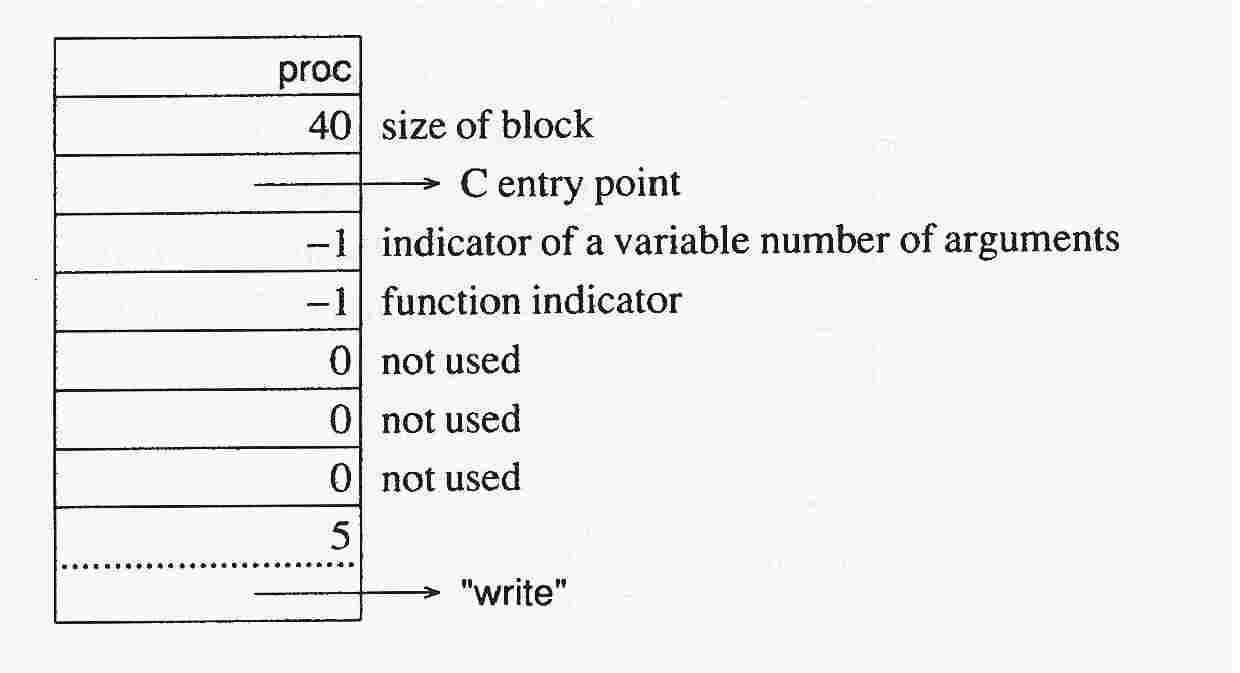
\includegraphics[width=4.1681in,height=2.248in]{ib-img/ib-img125.jpg} 
\begin{picture}(300,170)
\begin{picture}(0,0)(-100,-32)
\put(0,0){\blkbox{0}{0}}
\put(0,0){\rightboxlabels{not used}{not used}}
\put(0,32){\blkbox{-1}{0}}
\put(0,32){\rightboxlabels{function indicator}{not used}}
\put(0,64){\wordbox{-1}{}}
\put(0,64){\brboxlabel{indicator of a variable number of arguments}}
\put(0,80){\blkptrbox{40}{40}{C entry point}}
\put(0,80){\trboxlabel{size of block}}
\put(0,112){\wordbox{proc}{}}
\end{picture}
\put(100,0){\dvptrbox{5}{}{40}{"write"}}
\end{picture}

\subsection{A.2.8 Files}

The block for a file contains a pointer to the corresponding file, a
word containing the file status, and a qualifier for the name of the
file. For example, the block for \texttt{\&output} is


%--%\ \  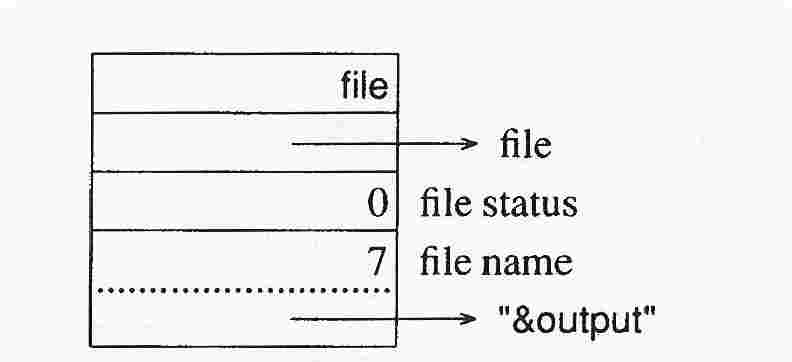
\includegraphics[width=2.6717in,height=1.2083in]{ib-img/ib-img126.jpg} 
\begin{picture}(300,100)
\put(120,0){\dvptrbox{7}{}{40}{\texttt{"\&output"}}}
\put(120,0){\trboxlabel{file name}}
\put(120,32){\wordbox{2}{}}
\put(120,32){\brboxlabel{file status}}
\put(120,48){\blkptrbox{file}{40}{file}}
\put(0,64){\dvptrbox{file}{np}{40}{}}
\end{picture}


The file status values are

\begin{tabular}{l@{\hspace{1cm}}l}
0 & closed\\
1 & open for reading\\
2 & open for writing\\
4 & open to create\\
8 & open to append\\
16 & open as a pipe\\
\end{tabular}

\subsection{A.2.9 Trapped Variables}

There are three kinds of trapped variables: keyword trapped variables,
substring trapped variables, and table-element trapped variables. The
corresponding blocks are tailored to the kind of trapped variable.


The value of \texttt{\&trace} illustrates a typical keyword trapped variable:


%--%\ \  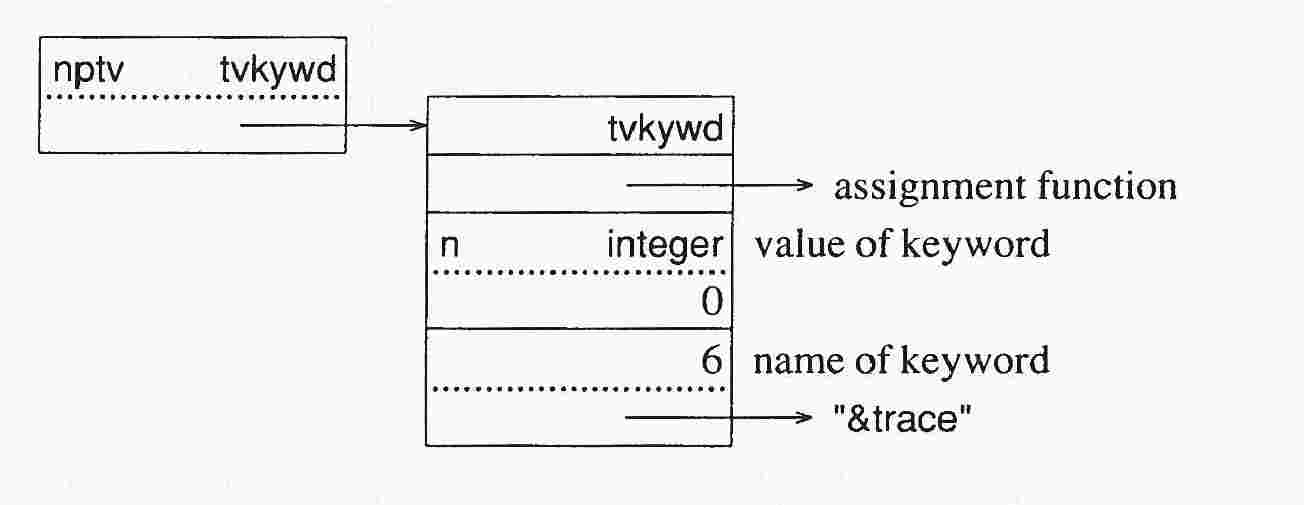
\includegraphics[width=4.3811in,height=1.6862in]{ib-img/ib-img127.jpg} 
\begin{picture}(300,120)(-20,0)
\put(0,80){\dvptrbox{tvkywd}{nptv}{60}{}}
\put(140,64){\blkptrbox{tvkywd}{50}{assignment function}}
\put(140,32){\dvbox{integer}{n}{0}}
\put(140,32){\trboxlabel{value of keyword}}
\put(140,0){\dvptrbox{6}{}{50}{"\&trace"}}
\end{picture}


A substring trapped variable contains the offset and length of the
substring, as well as a variable that points to the qpalifier for the
string. For example, if the value of \texttt{s} is
{\textquotedbl}abcdef{\textquotedbl}, the substring trapped-variable
block for \texttt{s[2:5]} is


%--%\ \  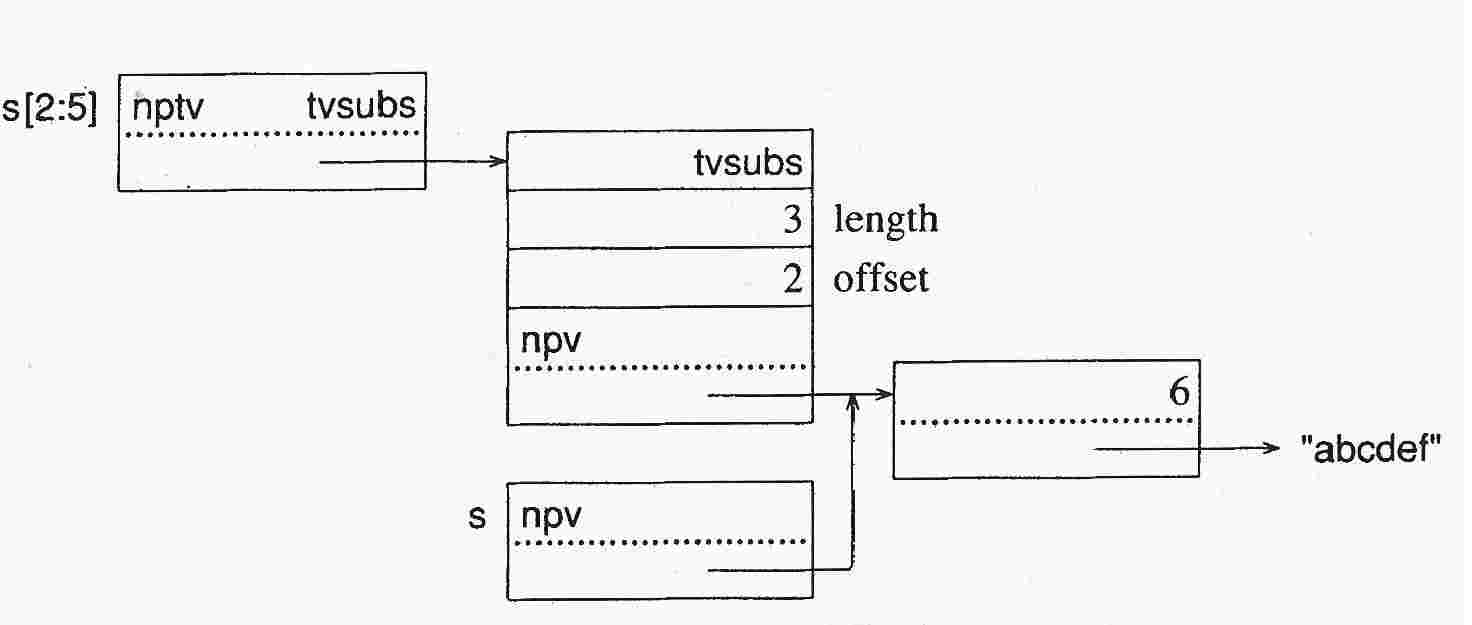
\includegraphics[width=4.9161in,height=2.0866in]{ib-img/ib-img128.jpg} 
\begin{picture}(300,170)
\put(140,0){\dvbox{}{npv}{}}
\put(140,0){\tlboxlabel{\texttt{s}}}
\put(140,0){\ruptr{30}{48}}
\put(140,48){\dvptrbox{}{npv}{50}{}}
\put(140,80){\blkbox{3}{2}}
\put(140,80){\rightboxlabels{length}{offset}}
\put(140,112){\wordbox{tvsubs}{}}
\put(10,112){\dvptrbox{tvsubs}{nptv}{50}{}}
\put(10,112){\tlboxlabel{\texttt{s[2:5]}}}
\put(260,32){\dvptrbox{6}{}{50}{\texttt{"abcdef"}}}
\end{picture}


A table-element trapped-variable block contains a word for the hash
number of the entry value, a pointer to the table, the entry value,
and a descriptor reserved for the assigned value. For example, if \texttt{t} is
a table, the table-element trapped-variable block for \texttt{t[36]} is


%--%\ \  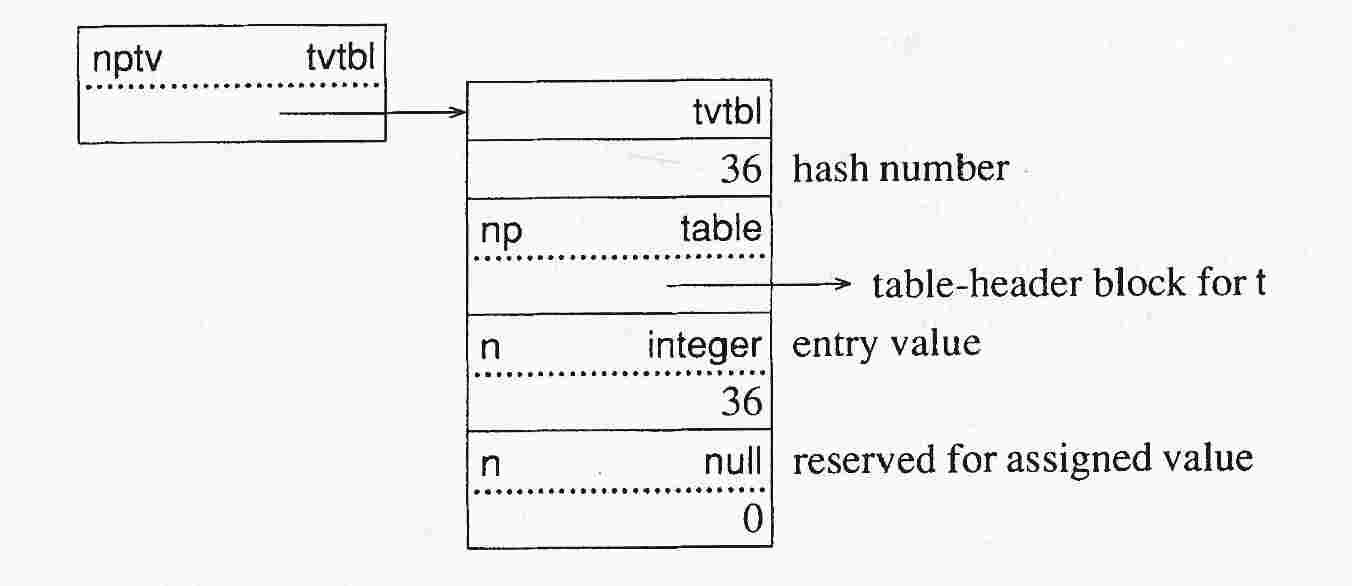
\includegraphics[width=4.5953in,height=1.9571in]{ib-img/ib-img129.jpg} 
\begin{picture}(300,150)
\put(120,0){\dvbox{null}{n}{0}}
\put(120,0){\trboxlabel{reserved for assigned value}}
\put(120,32){\dvbox{integer}{n}{36}}
\put(120,32){\trboxlabel{entry value}}
\put(120,64){\dvptrbox{table}{np}{40}{table header block for t}}
\put(120,96){\blkbox{tvtbl}{36}}
\put(120,96){\brboxlabel{hash number}}
\put(0,112){\dvptrbox{tvtbl}{nptv}{40}{}}
\end{picture}

\subsection{A.2.10 Co-Expressions}

A co-expression block consists of heading information, an array of
words for saving the C state, an interpreter stack, and a C stack:

%--%\ \  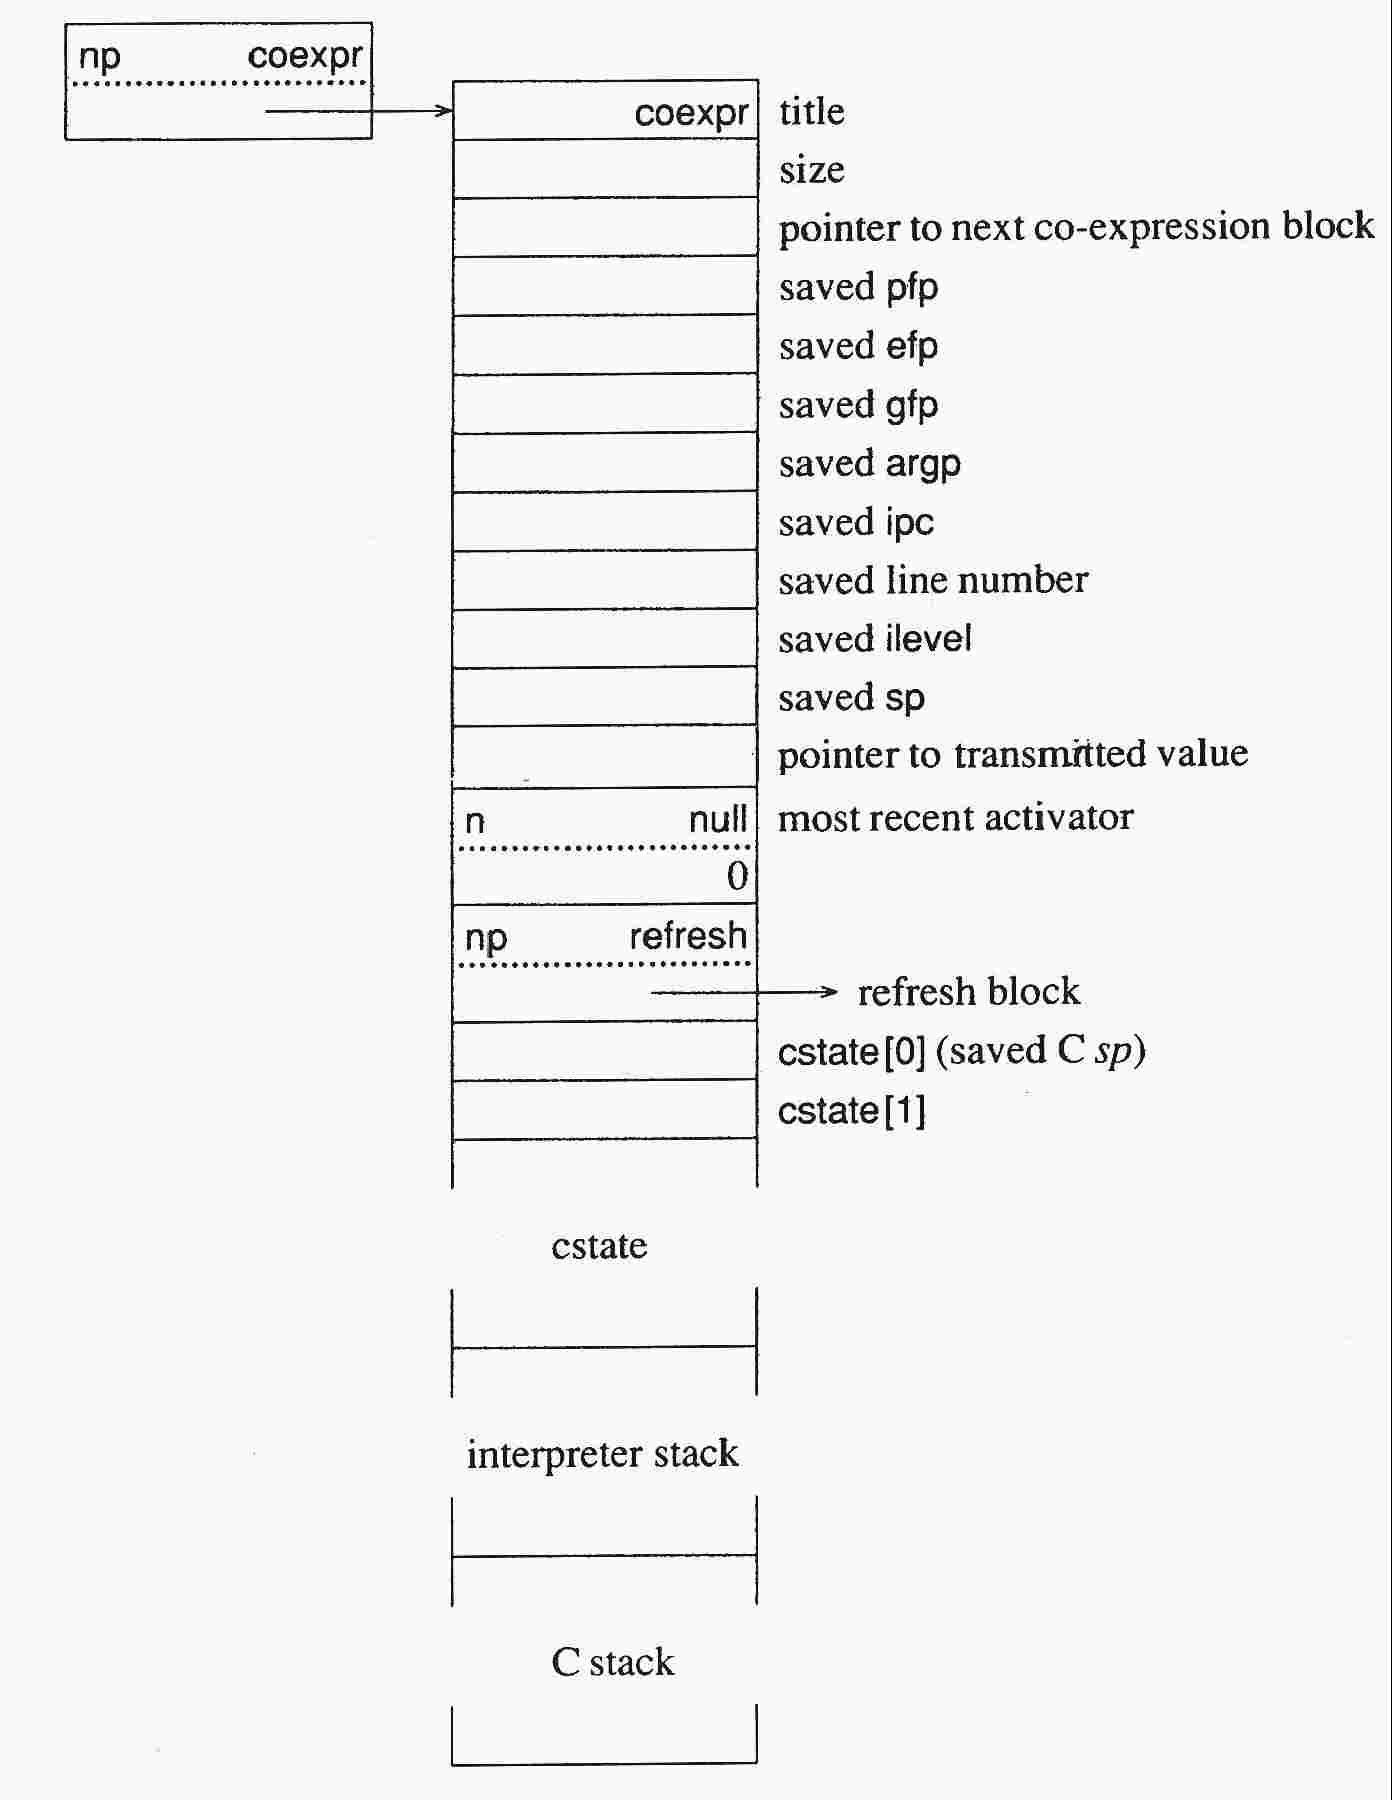
\includegraphics[width=4.702in,height=6.0126in]{ib-img/ib-img130.jpg} 
\begin{picture}(300,440)
\put(104,10){\makebox[100pt]{C stack}}
\put(100,32){\updownbars}
\put(104,52){\makebox[100pt]{interpreter stack}}
\put(100,80){\updownbars}
\put(104,100){\makebox[100pt]{cstate}}
\put(100,136){\downbars}
\put(100,136){\blkbox{}{}}
\put(100,136){\rightboxlabels{cstate[0] (saved C {\em sp})}{cstate[1]}}
\put(100,168){\dvptrbox{refresh}{np}{40}{refresh block}}
\put(100,200){\dvbox{null}{n}{0}}
\put(100,200){\trboxlabel{most recent activator}}
\put(100,232){\blkbox{}{}}
\put(100,232){\rightboxlabels{saved sp}{pointer to transmitted value}}
\put(100,264){\blkbox{}{}}
\put(100,264){\rightboxlabels{saved line number}{saved ilevel}}
\put(100,296){\blkbox{}{}}
\put(100,296){\rightboxlabels{saved argp}{saved ipc}}
\put(100,328){\blkbox{}{}}
\put(100,328){\rightboxlabels{saved efp}{saved gfp}}
\put(100,360){\blkbox{}{}}
\put(100,360){\rightboxlabels{pointer to next co-expression block}{saved pfp}}
\put(100,392){\blkbox{coexpr}{}}
\put(100,392){\rightboxlabels{title}{size}}
\put(-20,408){\dvptrbox{coexpr}{np}{40}{}}
\end{picture}


The refresh block contains information derived from the procedure
block for the procedure in which the co-expression was
created. Consider, for example,

%-% {\ttfamily\mdseries
%-% \ \ procedure labgen(s)}
%-% 
%-% {\ttfamily\mdseries
%-% \ \ local i, j, e}
%-% 
%-% {\ttfamily\mdseries
%-% \ \ i := 1}
%-% 
%-% {\ttfamily\mdseries
%-% \ \ j := 100}
%-% 
%-% {\ttfamily\mdseries
%-% \ \ e := create (s {\textbar}{\textbar} (i to j) {\textbar}{\textbar} {\textquotedbl}:{\textquotedbl})}
%-% 
%-% {\ttfamily\mdseries
%-% \ \ ...}
%-% 
%-% {\ttfamily\mdseries
%-% \ \ end}
\goodbreak
\iconcode{
procedure labgen(s)\\
\>local i, j, e\\
\>i := 1\\
\>j := 100\\
\>e := create (s || (i to j) || ":")\\
\>\>\vdots\\
end
}

For the call labgen({\textquotedbl}L{\textquotedbl}), the refresh block for \texttt{e} is

%--%\ \  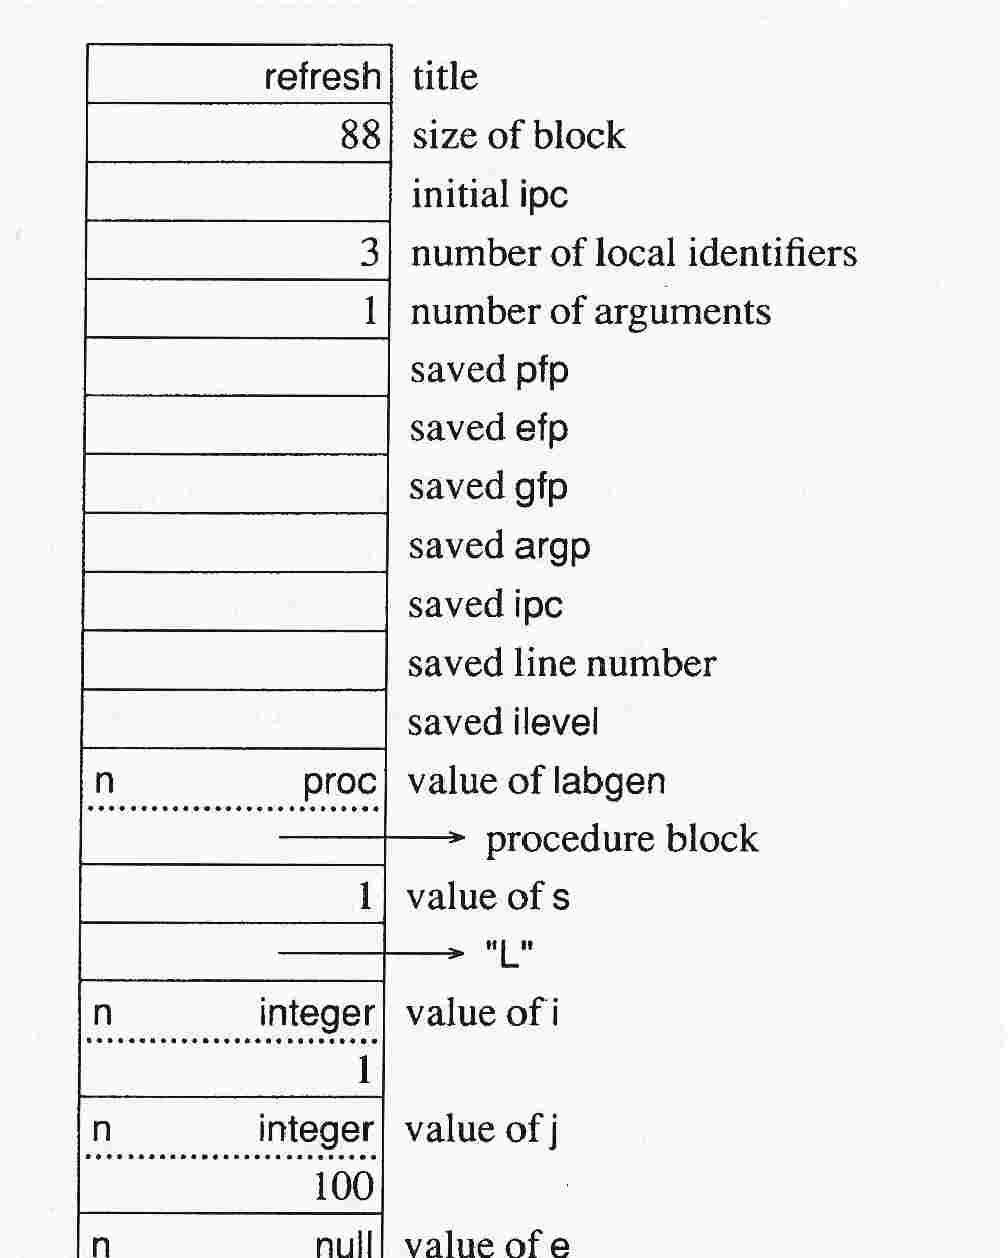
\includegraphics[width=3.4193in,height=4.2016in]{ib-img/ib-img131.jpg} 
\begin{picture}(300,380)
\put(100,0){\dvbox{null}{n}{0}}
\put(100,0){\trboxlabel{value of e}}
\put(100,32){\dvbox{integer}{n}{100}}
\put(100,32){\trboxlabel{value of j}}
\put(100,64){\dvbox{null}{n}{1}}
\put(100,64){\trboxlabel{value of i}}
\put(100,96){\dvptrbox{1}{}{40}{"L"}}
\put(100,96){\trboxlabel{value of s}}
\put(100,128){\dvptrbox{proc}{n}{40}{procedure block}}
\put(100,128){\trboxlabel{value of labgen}}
\put(100,160){\blkbox{}{}}
\put(100,160){\rightboxlabels{saved line number}{saved ilevel}}
\put(100,192){\blkbox{}{}}
\put(100,192){\rightboxlabels{saved argp}{saved ipc}}
\put(100,224){\blkbox{}{}}
\put(100,224){\rightboxlabels{saved efp}{saved gfp}}
\put(100,256){\blkbox{}{}}
\put(100,256){\rightboxlabels{saved number of arguments}{saved pfp}}
\put(100,288){\blkbox{}{3}}
\put(100,288){\rightboxlabels{initial ipc}{number of local identifiers}}
\put(100,320){\blkbox{refresh}{88}}
\put(100,320){\rightboxlabels{title}{size of block}}
\end{picture}
